% Options for packages loaded elsewhere
\PassOptionsToPackage{unicode}{hyperref}
\PassOptionsToPackage{hyphens}{url}
\PassOptionsToPackage{dvipsnames,svgnames,x11names}{xcolor}
%
\documentclass[
  singlecolumn]{article}

\usepackage{amsmath,amssymb}
\usepackage{iftex}
\ifPDFTeX
  \usepackage[T1]{fontenc}
  \usepackage[utf8]{inputenc}
  \usepackage{textcomp} % provide euro and other symbols
\else % if luatex or xetex
  \usepackage{unicode-math}
  \defaultfontfeatures{Scale=MatchLowercase}
  \defaultfontfeatures[\rmfamily]{Ligatures=TeX,Scale=1}
\fi
\usepackage[]{libertinus}
\ifPDFTeX\else  
    % xetex/luatex font selection
\fi
% Use upquote if available, for straight quotes in verbatim environments
\IfFileExists{upquote.sty}{\usepackage{upquote}}{}
\IfFileExists{microtype.sty}{% use microtype if available
  \usepackage[]{microtype}
  \UseMicrotypeSet[protrusion]{basicmath} % disable protrusion for tt fonts
}{}
\makeatletter
\@ifundefined{KOMAClassName}{% if non-KOMA class
  \IfFileExists{parskip.sty}{%
    \usepackage{parskip}
  }{% else
    \setlength{\parindent}{0pt}
    \setlength{\parskip}{6pt plus 2pt minus 1pt}}
}{% if KOMA class
  \KOMAoptions{parskip=half}}
\makeatother
\usepackage{xcolor}
\usepackage[top=30mm,left=20mm,heightrounded]{geometry}
\setlength{\emergencystretch}{3em} % prevent overfull lines
\setcounter{secnumdepth}{-\maxdimen} % remove section numbering
% Make \paragraph and \subparagraph free-standing
\ifx\paragraph\undefined\else
  \let\oldparagraph\paragraph
  \renewcommand{\paragraph}[1]{\oldparagraph{#1}\mbox{}}
\fi
\ifx\subparagraph\undefined\else
  \let\oldsubparagraph\subparagraph
  \renewcommand{\subparagraph}[1]{\oldsubparagraph{#1}\mbox{}}
\fi


\providecommand{\tightlist}{%
  \setlength{\itemsep}{0pt}\setlength{\parskip}{0pt}}\usepackage{longtable,booktabs,array}
\usepackage{calc} % for calculating minipage widths
% Correct order of tables after \paragraph or \subparagraph
\usepackage{etoolbox}
\makeatletter
\patchcmd\longtable{\par}{\if@noskipsec\mbox{}\fi\par}{}{}
\makeatother
% Allow footnotes in longtable head/foot
\IfFileExists{footnotehyper.sty}{\usepackage{footnotehyper}}{\usepackage{footnote}}
\makesavenoteenv{longtable}
\usepackage{graphicx}
\makeatletter
\def\maxwidth{\ifdim\Gin@nat@width>\linewidth\linewidth\else\Gin@nat@width\fi}
\def\maxheight{\ifdim\Gin@nat@height>\textheight\textheight\else\Gin@nat@height\fi}
\makeatother
% Scale images if necessary, so that they will not overflow the page
% margins by default, and it is still possible to overwrite the defaults
% using explicit options in \includegraphics[width, height, ...]{}
\setkeys{Gin}{width=\maxwidth,height=\maxheight,keepaspectratio}
% Set default figure placement to htbp
\makeatletter
\def\fps@figure{htbp}
\makeatother
\newlength{\cslhangindent}
\setlength{\cslhangindent}{1.5em}
\newlength{\csllabelwidth}
\setlength{\csllabelwidth}{3em}
\newlength{\cslentryspacingunit} % times entry-spacing
\setlength{\cslentryspacingunit}{\parskip}
\newenvironment{CSLReferences}[2] % #1 hanging-ident, #2 entry spacing
 {% don't indent paragraphs
  \setlength{\parindent}{0pt}
  % turn on hanging indent if param 1 is 1
  \ifodd #1
  \let\oldpar\par
  \def\par{\hangindent=\cslhangindent\oldpar}
  \fi
  % set entry spacing
  \setlength{\parskip}{#2\cslentryspacingunit}
 }%
 {}
\usepackage{calc}
\newcommand{\CSLBlock}[1]{#1\hfill\break}
\newcommand{\CSLLeftMargin}[1]{\parbox[t]{\csllabelwidth}{#1}}
\newcommand{\CSLRightInline}[1]{\parbox[t]{\linewidth - \csllabelwidth}{#1}\break}
\newcommand{\CSLIndent}[1]{\hspace{\cslhangindent}#1}

\usepackage{booktabs}
\usepackage{longtable}
\usepackage{array}
\usepackage{multirow}
\usepackage{wrapfig}
\usepackage{float}
\usepackage{colortbl}
\usepackage{pdflscape}
\usepackage{tabu}
\usepackage{threeparttable}
\usepackage{threeparttablex}
\usepackage[normalem]{ulem}
\usepackage{makecell}
\usepackage{xcolor}
\usepackage{cancel}
\usepackage[noblocks]{authblk}
\renewcommand*{\Authsep}{, }
\renewcommand*{\Authand}{, }
\renewcommand*{\Authands}{, }
\renewcommand\Affilfont{\small}
\usepackage{cancel}
\makeatletter
\makeatother
\makeatletter
\makeatother
\makeatletter
\@ifpackageloaded{caption}{}{\usepackage{caption}}
\AtBeginDocument{%
\ifdefined\contentsname
  \renewcommand*\contentsname{Table of contents}
\else
  \newcommand\contentsname{Table of contents}
\fi
\ifdefined\listfigurename
  \renewcommand*\listfigurename{List of Figures}
\else
  \newcommand\listfigurename{List of Figures}
\fi
\ifdefined\listtablename
  \renewcommand*\listtablename{List of Tables}
\else
  \newcommand\listtablename{List of Tables}
\fi
\ifdefined\figurename
  \renewcommand*\figurename{Figure}
\else
  \newcommand\figurename{Figure}
\fi
\ifdefined\tablename
  \renewcommand*\tablename{Table}
\else
  \newcommand\tablename{Table}
\fi
}
\@ifpackageloaded{float}{}{\usepackage{float}}
\floatstyle{ruled}
\@ifundefined{c@chapter}{\newfloat{codelisting}{h}{lop}}{\newfloat{codelisting}{h}{lop}[chapter]}
\floatname{codelisting}{Listing}
\newcommand*\listoflistings{\listof{codelisting}{List of Listings}}
\makeatother
\makeatletter
\@ifpackageloaded{caption}{}{\usepackage{caption}}
\@ifpackageloaded{subcaption}{}{\usepackage{subcaption}}
\makeatother
\makeatletter
\@ifpackageloaded{tcolorbox}{}{\usepackage[skins,breakable]{tcolorbox}}
\makeatother
\makeatletter
\@ifundefined{shadecolor}{\definecolor{shadecolor}{rgb}{.97, .97, .97}}
\makeatother
\makeatletter
\makeatother
\makeatletter
\makeatother
\ifLuaTeX
  \usepackage{selnolig}  % disable illegal ligatures
\fi
\IfFileExists{bookmark.sty}{\usepackage{bookmark}}{\usepackage{hyperref}}
\IfFileExists{xurl.sty}{\usepackage{xurl}}{} % add URL line breaks if available
\urlstyle{same} % disable monospaced font for URLs
\hypersetup{
  pdftitle={Causal inference in three wave panels: a step-by-step guide},
  pdfauthor={Joseph A. Bulbulia},
  pdfkeywords={DAGS, Causal
Inference, Confounding, History, Psychology, Panel},
  colorlinks=true,
  linkcolor={blue},
  filecolor={Maroon},
  citecolor={Blue},
  urlcolor={Blue},
  pdfcreator={LaTeX via pandoc}}

\title{Causal inference in three wave panels: a step-by-step guide}


  \author{Joseph A. Bulbulia}
            \affil{%
                  Victoria University of Wellington, New Zealand, School
                  of Psychology, Centre for Applied Cross-Cultural
                  Research
              }
      
\date{2023-08-11}
\begin{document}
\maketitle
\begin{abstract}
How to estimate causal effects in three wave panel designs
\end{abstract}
\ifdefined\Shaded\renewenvironment{Shaded}{\begin{tcolorbox}[breakable, interior hidden, enhanced, sharp corners, borderline west={3pt}{0pt}{shadecolor}, boxrule=0pt, frame hidden]}{\end{tcolorbox}}\fi

\hypertarget{introduction}{%
\subsection{Introduction}\label{introduction}}

\hypertarget{purpose}{%
\subsubsection{Purpose}\label{purpose}}

I describe how to calculate causal effects in three-wave panel designs.

\textbf{Part 1} introduces definitions and notation.

\textbf{Part 2} describes the three-wave panel, and its motivations.

\textbf{Part 3} develops a the step-by-step guide for conducting causal
inference within the three-wave panel design

\textbf{Part 4} describes common estimators

\textbf{Part 5} discusses more complex designs where there is scope for
confounder treatment feedback.

An Appendix describes custom functions I have written for executing the
workflows.

\hypertarget{part-1-definitions-and-notation}{%
\subsection{\texorpdfstring{\textbf{Part 1} Definitions and
notation}{Part 1 Definitions and notation}}\label{part-1-definitions-and-notation}}

\hypertarget{treatment-or-exposure}{%
\paragraph{\texorpdfstring{\textbf{Treatment or
Exposure}}{Treatment or Exposure}}\label{treatment-or-exposure}}

A treatment or exposure, denoted by \(A\), represents an intervention or
condition in a study. We assume that it can take different levels such
that \((A = a) \neq (A = a')\), which correspond to different states or
intensities of the intervention.

In plain terms, the treatment is the ``cause.''

\hypertarget{potential-or-counterfactual-outcomes}{%
\paragraph{\texorpdfstring{\textbf{Potential or Counterfactual
Outcomes}}{Potential or Counterfactual Outcomes}}\label{potential-or-counterfactual-outcomes}}

Potential or counterfactual outcomes, denoted by \(Y\), represent the
values that an outcome would take on if a treatment or exposure were,
perhaps contrary to fact, set to a specific level
(\protect\hyperlink{ref-ogburn2021}{Ogburn and Shpitser 2021}).

We use the terms ``potential outcomes'' and ``counterfactual outcomes''
synonymously.

We denote a potential outcome using the notation \(Y(A = a)\) or simply
\(Y(a)\).

\hypertarget{causal-contrast}{%
\paragraph{\texorpdfstring{\textbf{Causal
Contrast}}{Causal Contrast}}\label{causal-contrast}}

A causal contrast is a function that quantifies a difference, at some
scale, in potential outcomes under different treatment levels.

Formally, a causal contrast is a function of potential outcomes:

\[f_{\text{causal contrast}}(Y(a), Y(a'))\]

where \(Y(a)\) and \(Y(a')\) represent the potential outcomes under the
specific treatment levels \(A = a\) and \(A = a'\), respectively.

Where \(ATE\) denotes the average treatment effect, a causal contrast on
the difference scale may be expressed:

\[ATE_{A,A'} = E[Y(a)] - E[Y(a')]\]

This essentially denotes an average treatment effect comparing the
outcome under treatment level \(A\) to the outcome under treatment level
\(A'\). For all exposures, including continuous exposures, we must
stipulate the level of contrast for the treatment.

Likewise we may state the average treatment effect on the ratio scale

\[ATE_{A/A'} = \frac{E[Y(a)]}{E[Y(a')]}\]

\hypertarget{causal-effect}{%
\paragraph{\texorpdfstring{\textbf{Causal
Effect}}{Causal Effect}}\label{causal-effect}}

We say there is a causal effect on the difference scale when a causal
estimand does not equal zero, indicating that the exposure influences
the outcome. For example:

\[E[Y(a)] - E[Y(a')] \neq 0\]

We say there is a causal effect on the ratio scale when a causal
estimand does not equal one. For example:

\[\frac{E[Y(1)]}{E[Y(0)]}\neq 1\]

where 1 and 0 represent specific levels of a binary exposure.

\hypertarget{observed-association}{%
\paragraph{\texorpdfstring{\textbf{Observed
Association}}{Observed Association}}\label{observed-association}}

The observed association is the measurable link between a treatment or
exposure \(A\) and an outcome \(Y\) in the sample data. We can represent
it as:

\[f_{\text{observed}}(Y, A)\]

For example, we may quantify an association between a treatment and
outcome using linear regression:

\[Y = \beta_0 + \beta_1 A + \epsilon\]

Where:

\begin{itemize}
\tightlist
\item
  \(Y\) is the outcome
\item
  \(A\) is the treatment or exposure
\item
  \(\beta_0\) and \(\beta_1\) are coefficients estimating the
  relationship
\item
  \(\epsilon\) is the error term
\end{itemize}

The slope (\(\beta_1\)) and intercept (\(\beta_0\)) estimates, obtained
using ordinary least squares (OLS), describe a relationship modelled as
linear.

\hypertarget{full-data-and-observed-data}{%
\paragraph{\texorpdfstring{\textbf{Full Data and Observed
Data}}{Full Data and Observed Data}}\label{full-data-and-observed-data}}

The full data is the random vector \((Y(1), Y(0), X, L)\) for covariates
\(L\), while the observed data \((Y, X, C)\) is a coarsening of the full
data with \(Y = X \cdot Y(1) + (1-X) \cdot Y(0)\)
(\protect\hyperlink{ref-ogburn2021}{Ogburn and Shpitser 2021}).

Absent assumptions, we cannot learn about causal estimands from the
observed data, because they are functionals of (partially) unobserved
potential outcomes.

\hypertarget{confounding}{%
\paragraph{\texorpdfstring{\textbf{Confounding}}{Confounding}}\label{confounding}}

A condition in which the observed association between the treatment and
the outcome in the data does not reflect a causal association.

\hypertarget{confounder}{%
\paragraph{\texorpdfstring{\textbf{Confounder}}{Confounder}}\label{confounder}}

Any variable that when conditioned upon, perhaps in conjunction with
other confounders, reduces or minimises confounding. In the scientific
investigation of causality, one must often grapple with confounders.
These may be categorised into two distinct types:

\begin{itemize}
\item
  \textbf{Measured Confounder} (\(L\)): A variable that has been
  meticulously documented in the study. The symbol \(L\) is used to
  represent this kind of confounder, and it is a variable that has
  influence on both the treatment and the outcome of interest. By
  incorporating this information into the analysis, researchers can
  diminish or eradicate bias in the causal estimation.
\item
  \textbf{Unmeasured Confounder} (\(U\)): Represented by the symbol
  \(U\), an unmeasured confounder is a variable that is influential on
  both the treatment and the outcome but, regrettably, has not been
  captured in the study's data. The inability to control for \(U\) can
  potentially introduce an erroneous bias in the estimation of the
  causal relationship, a situation that can complicate the understanding
  of true causal effects. This scenario is a subject of considerable
  concern, especially in observational studies where information on all
  confounders might not be attainable.
\end{itemize}

\hypertarget{causal-estimand}{%
\paragraph{\texorpdfstring{\textbf{Causal
Estimand}}{Causal Estimand}}\label{causal-estimand}}

A causal estimand names the causal contrast of interest, specifying the
levels of exposure to be contrasted, potential outcomes of interest, the
scale of the causal contrast, and the target population for whom the
causal contrast applies.

\hypertarget{statistical-estimand}{%
\paragraph{\texorpdfstring{\textbf{Statistical
Estimand}}{Statistical Estimand}}\label{statistical-estimand}}

A statistical estimand is a functional of the observed data that
corresponds to the causal estimand of interest. It reduces the causal
question to a statistical one, identifying a quantity in the observed
data that will provide information about the causal estimand.

\hypertarget{estimator}{%
\paragraph{\texorpdfstring{\textbf{Estimator}}{Estimator}}\label{estimator}}

An estimator is a statistical function of the observed data, denoted as
\(\hat{\theta}(Y, A, L)\), that provides an estimate of the statistical
estimand. It translates the observed data into a single value,
approximating the unknown parameter. In the context of causal inference,
an estimator is used to estimate the statistical estimand, thereby
providing information about the corresponding causal estimand.

\hypertarget{source-population}{%
\paragraph{\texorpdfstring{\textbf{Source
Population}}{Source Population}}\label{source-population}}

A source population is the population from who a study sample is drawn.

\hypertarget{target-population}{%
\paragraph{\texorpdfstring{\textbf{Target
Population}}{Target Population}}\label{target-population}}

A target population is the larger group we aim to apply our study's
results to. It could be defined by location, demographics, or specific
conditions.

The closer the source matches the target in ways that are relevant to
our causal questions, the stronger our causal inferences about the
target population will be.

\hypertarget{generalisability}{%
\paragraph{\texorpdfstring{\textbf{Generalisability}}{Generalisability}}\label{generalisability}}

We say our results generalise when the causal effect estimated from a
sample apply to the wider population from was drawn from the sample
population. This is ``external validity.'' Where \(PATE\) denotes the
population average treatement effect:

\[\text{Generalisability} = PATE \approx f(ATE_{\text{sample}}, W)\]

\hypertarget{transportability}{%
\paragraph{\texorpdfstring{\textbf{Transportability}}{Transportability}}\label{transportability}}

We say our results are transportable when the causal effect estimated
from a sample apply to a population other than that from which the
sample population is drawn. This can be expressed:

\[\text{Transportability} = ATE_{\text{target}} \approx f(ATE_{\text{source}}, T)\]

where \(f\) is a function and \(T\) is a function that maps the results
from our source population to another population.

To achieve transportability, we need information about the source and
target populations and an understanding of how the relationships between
treatment, outcome, and covariates differ between the populations. That
is assessing transportability requires scientific knowledge.

\hypertarget{elicitation}{%
\paragraph{\texorpdfstring{\textbf{Elicitation}}{Elicitation}}\label{elicitation}}

Elicitation refers to the process of gathering expert opinion or
knowledge to inform a model or analysis. We shall see the importance of
elicitation throughout.

\hypertarget{experiments}{%
\subsubsection{Experiments}\label{experiments}}

\hypertarget{average-causal-effects-in-experiments}{%
\subsubsection{\texorpdfstring{\textbf{Average Causal Effects in
Experiments}}{Average Causal Effects in Experiments}}\label{average-causal-effects-in-experiments}}

Estimating a causal effect means comparing what actually happened to
what would have happened if things had been different.

In an experiment, we place people into groups, give a treatment, and
then see what happens. But we can never see what would have happened to
a person in a different group. We only see what happens in the group
they were placed in.

When we talk about average effects of a treatment, things are different.
In a perfect experiment, we can compare the groups because we know the
assignment to groups is random. We can work out the average effect of
the treatment by comparing what generally happened in the treatment
group to what generally happened in the control group.

The random way we place people in groups means that, in theory, anyone
in one group could have been in the other. So, we can work out the
average effect without having to know exactly what would have happened
to each individual in both groups.

\hypertarget{conditional-causal-effects-in-experiments}{%
\paragraph{\texorpdfstring{\textbf{Conditional Causal Effects in
Experiments}}{Conditional Causal Effects in Experiments}}\label{conditional-causal-effects-in-experiments}}

The effect of a treatment might change based on factors such as age or
education.

In an experiment, we can study people who are similar in some way, like
being the same age. We compare how the treatment works for them against
a control group without the treatment.

This is a conditional causal effect. It tells us how the treatment might
work for certain groups of people. It helps us understand who the
treatment helps the most.

Randomisation is essential here, too. Because we put people into groups
randomly, we can trust that differences in how the groups respond, on
average, owe to the treatment, not to other factors. We do not need to
guess what would have happened members of a different group had they
been assigned to a different condition. Random assignment enables us to
compute group-level responses within conditions, bypassing the need to
observe what cannot, in reality, ever be observed -- individual-level
contrasts.

\hypertarget{estimating-causal-effects-outside-of-experiments-requires-assumptions}{%
\paragraph{\texorpdfstring{\textbf{Estimating Causal Effects outside of
Experiments Requires
Assumptions}}{Estimating Causal Effects outside of Experiments Requires Assumptions}}\label{estimating-causal-effects-outside-of-experiments-requires-assumptions}}

Experiments are the best method for estimating causal effects. They use
randomisation and control to identify causation. However, experiments
are not always possible or ethical. In those cases, researchers turn to
observational studies. These studies are more complex. They do not have
random assignment to treatment conditions, and the conditions may vary
widely. Some individuals might not even have a chance to receive one or
both levels of the treatment being studied.

Therefore, to estimate causal effects in observational settings, certain
assumptions must be met {[}citations{]}. These assumptions are crucial.
Without them, it is risky to draw conclusions about causation outside of
experimental settings {[}cite{]}.

The three fundamental assumptions are the exchangeability assumption,
the causal consistency assumption, and the positivity assumption. Each
one serves a unique role in ensuring that the causal effects identified
in observational studies are valid and reliable.

\hypertarget{the-exchangeability-assumption}{%
\paragraph{\texorpdfstring{\textbf{The Exchangeability
Assumption}}{The Exchangeability Assumption}}\label{the-exchangeability-assumption}}

In observational studies, the lack of randomisation can lead to
challenges in identifying causal effects.

Specifically, the assumption requires that, after controlling for
measured variables, the potential outcomes under various exposure levels
must be independent of the actual exposure level experienced
(\protect\hyperlink{ref-hernuxe1n2023}{Hernán and Monge 2023}).

The exchangeability assumption addresses this issue. It requires balance
in the treatment conditions, considering factors that might influence
the outcome. When the data do have balance across the treatment
conditions, we say there is ``confounding.'' The task is removing
confounding is one of obtaining balance of the kind that randomisation
provides in experimental settings.

In the following sections, we will outline methods for addressing the
exchangeability assumption. Because the data do not typically clarify
whether counfounding has been fully addressed, we recommend sensitivity
analysis. Such analyses describe how much unmeasured confounding would
be required to explain away the observed association between the
exposure and the outcome.

\hypertarget{the-causal-consistency-assumption}{%
\paragraph{\texorpdfstring{\textbf{The Causal Consistency
Assumption}}{The Causal Consistency Assumption}}\label{the-causal-consistency-assumption}}

In observational studies, researchers lack control over the treatment,
creating complexity in discerning causal effects.

The causal consistency assumption helps navigate this complexity. It
mandates that the exposures being compared align with specific,
well-defined interventions in the data
(\protect\hyperlink{ref-hernuxe1n2023}{Hernán and Monge 2023}).

This means that the exposure or treatment must be consistent across the
study, and it should not change over time or vary among subjects in ways
that might alter the outcome (see also: Chatton \emph{et al.}
(\protect\hyperlink{ref-chatton2020}{2020})).

Consider a multifaceted ``treatment'' such as weight loss. In real-world
weight loss, various means may be employed: dieting, exercise, stress,
severe disease, surgical procedures like stomach stapling. Each
constitutes a different exposure with unique effects.

In experiments, experimental control allows us to define the exposure
precisely, such as weight loss by dieting. By controlling other factors,
we can isolate the causal effect of that specific intervention. In this
scenario, the causal consistency assumption is satisfied because the
intervention does not vary in ways that would affect the result.

In observational studies, ensuring causal consistency becomes more
challenging. Studies might include individuals losing weight through
various means, with differing motivations, methods, and individual
characteristics (\protect\hyperlink{ref-tyler}{\textbf{tyler?}}).
Without control over these factors, the causal consistency assumption
may be violated, complicating the isolation of a specific intervention's
effect like dieting.

Though estimating causal effects in heterogeneous treatment settings is
complex, it is not incoherent. A mathematical framework, known as causal
inference under multiple versions of treatment, shows that unbiased
estimation is feasible if all treatment versions meet the
exchangeability assumption. Practical challenges do arise, though.
Without observing the many versions of treatment, evaluating the
exchangeability assumption may become difficult, and the utility of the
estimation can be limited. For example, estimating the effect of weight
loss through a random assignment to either dieting or heart disease may
provide little meaningful insight due to the heterogeneous nature of the
treatments.

Unfortunately, the causal consistency assumption typically cannot be
verified by inspecting the data. Rather, researchers must rely on a
clear understanding of the subject matter, make informed decisions about
the definitions of exposures and treatments, and use thorough study
design and statistical methods. They must ensure that the exposure or
intervention being studied is consistently defined and measured across
subjects in the study, without variation that could affect the outcome.
This often involves careful consideration of the context, consultation
with domain experts, and methodological choices that reflect the
underlying science of the phenomenon being studied.

The protocols we describe below are aimed to help researchers obtain
sensible inference by focussing their attention these demands for
contextual attention informed by expert advice.

\hypertarget{the-positivity-assumption}{%
\paragraph{\texorpdfstring{\textbf{The Positivity
Assumption}}{The Positivity Assumption}}\label{the-positivity-assumption}}

There is a non-zero probability of receiving every exposure value within
all strata of covariates (\protect\hyperlink{ref-hernuxe1n2023}{Hernán
and Monge 2023}).

In simpler terms, it means that every subject in the study has some
chance of receiving each level of the exposure or treatment.

If this assumption is not met, it becomes impossible to make meaningful
comparisons between different levels of exposure, as some of the
comparisons would be based on groups where the exposure was never
applied.

Unlike the exchangeability and causal consistency assumptions, we can
sometimes verify whether the positivity assumption is satisfied by
inspecting the data.

\hypertarget{identification-strategy}{%
\paragraph{\texorpdfstring{\textbf{Identification
Strategy}}{Identification Strategy}}\label{identification-strategy}}

An identification strategy refers to the set of assumptions and
methodologies employed to ensure that a causal estimand (recall -- a
quantity representing a causal effect) can be determined uniquely from
the observed data. It is the process through which researchers make a
bridge from the statistical estimand, derived from the observed data, to
the causal estimand that represents the actual causal effect of
interest. Identifiability relies on assumptions such as exchangeability,
positivity, and consistent measurement. The validity of these
assumptions enables a unique mapping of the causal estimand from the
statistical estimand, facilitating causal inference from observational
data.

Ide

\hypertarget{considerations}{%
\paragraph{Considerations}\label{considerations}}

\begin{itemize}
\tightlist
\item
  In the causal inference literature, the concept we use to make sense
  of stratum specific comparisons is called ``effect modification.''
\item
  By inferring effects within stratums, we may evaluate whether the
  effects of different exposures or treatments on some well-defined
  outcome (measured in some well-defined time-period after the exposure)
  differ depending on group measurement.
\item
  The logic of effect modification differs slightly from that of
  interaction.
\end{itemize}

\hypertarget{aside-extensions}{%
\paragraph{Aside: extensions}\label{aside-extensions}}

For continuous exposures, we must stipulate the level of contrast for
the exposure (e.g.~weekly versus monthly church attendance):

\[ATE_{A,A'} = E[Y(A) - Y(A')| L]\]

This essentially denotes an average treatment effect comparing the
outcome under treatment level \(A\) to the outcome under treatment level
\(A'\).

Likewise:

\[ATE_{A/A'} = \frac{E[Y(A)| L]}{E[Y(A')| L]}\]

This defines the contrast of \(A\) and \(A'\) on a ratio scale.

\hypertarget{f.-describe-the-populations-for-whom-the-intended-study-is-meant-to-generalise-by-distinguishing-between-source-and-target-populations.}{%
\paragraph{f.~Describe the population(s) for whom the intended study is
meant to generalise by distinguishing between source and target
populations.}\label{f.-describe-the-populations-for-whom-the-intended-study-is-meant-to-generalise-by-distinguishing-between-source-and-target-populations.}}

Consider the following concepts:

\hypertarget{part-2-three-wave-panel-designs}{%
\subsection{Part 2`: Three-Wave Panel
Designs}\label{part-2-three-wave-panel-designs}}

Our goal is to explain how researchers can use three waves of data to
satisfy the assumptions needed for causal inference.

Put differently, we aim to demonstrate how, with three waves of data,
researchers can emulate the conditions found in a randomised experiment
so that they may address causal questions outsider of experiments.

To begin, let us clarify some definitions:

\begin{itemize}
\item
  \textbf{Wave}: a wave is a time interval where measurements are taken.
  It is placed on a timeline, so there are earlier and later intervals.
  The length can vary, but the order is specific.
\item
  \textbf{Treatment (or Exposure)}: a treatment refers to an event or
  condition applied to some individuals but not others. In causal terms,
  it is what we consider the ``cause.'' Our discussion here will be
  limited to investigating the effects of one cause.
\item
  \textbf{Outcome}: an outcome is what we study as the effect of the
  treatment. It is the result we are interested in measuring.
\item
  \textbf{Confounding}: when the observed relationship between the
  treatment and the outcome may be influenced by another variable, not
  just the treatment itself, we say there may be confounding.
\item
  \textbf{Confounder}: a confounder is a variable that reduces
  confounding when it is accounted for in the study.
\item
  \textbf{Panel Design}: a panel design follows the same individuals
  over time. It enables baseline controls and connects treatments to
  outcomes.
\item
  \textbf{Baseline}: wave 0, or the baseline, is the interval in which
  we measure confounders to deal with confounding in a three-wave panel
  design.
\item
  \textbf{Treatment Wave}: wave 1 is the interval in which we measure
  the treatment or exposure is measured. Other variables at this wave
  are generally not included. However, we will explain how to address
  causal questions in which the effect of a treatment may vary between
  groups measured at baseline. That is, we will explain how to identify
  conditional causal effects.
\item
  \textbf{Outcome Wave}: wave 2 is the interval is the interval in which
  we measure, you guessed it, the outcome. There may be more than one
  outcome measured.
\end{itemize}

\hypertarget{step-1.-defining-the-exposure-measure-it-at-wave-0-and-wave-1}{%
\subsubsection{Step 1. Defining the exposure: measure it at wave 0 and
wave
1}\label{step-1.-defining-the-exposure-measure-it-at-wave-0-and-wave-1}}

We begin with a well-defined exposure.

Consider the causal effect of attending religious services. The first
critical step involves defining the exposure in the context of a
hypothetical intervention. What aspect is of interest to us? Is it a
comparison of attendance versus non-attendance? Are we distinguishing
between weekly and monthly attendees? Perhaps, we are interested in a
different facet altogether? Visualising a hypothetical experiment - even
when it is not feasible - reveals the need for a precise intervention
specification (\protect\hyperlink{ref-bulbulia2022}{Bulbulia 2022};
\protect\hyperlink{ref-hernuxe1n2016a}{Hernán \emph{et al.} 2016};
\protect\hyperlink{ref-hernuxe1n2022}{Hernán \emph{et al.} 2022}).

The exposure is measured at wave 1 (i.e.~+1 interval from baseline, wave
0). When estimating causal effects, the inclusion of exposure at the
baseline carries three critical advantages:

\begin{enumerate}
\def\labelenumi{\alph{enumi}.}
\tightlist
\item
  \textbf{Incidence effect interpretation}: incorporating the baseline
  exposure allows us to interpret the effect of exposure measured
  post-baseline as an incidence effect, not a prevalence effect
  (\protect\hyperlink{ref-vanderweele2020}{VanderWeele \emph{et al.}
  2020}). This means we can interpret the effect as the change due to a
  new occurrence (incidence) of the exposure, rather than the overall
  presence (prevalence) of the exposure. For example, in a study
  investigating the impact of weekly religious service attendance,
  including the baseline measure of attendance enables us to understand
  the effect of starting to attend weekly services (incidence), as
  opposed to simply being a regular attendee (prevalence).
\end{enumerate}

\begin{enumerate}
\def\labelenumi{\arabic{enumi}.}
\setcounter{enumi}{1}
\item
  \textbf{Confounding control}: the baseline exposure's inclusion helps
  to reduce unmeasured confounding arising from time-invariant
  confounders. These are variables that do not change over time and
  could confound the association between the exposure and the outcome if
  not properly accounted for. For instance, personal attributes such as
  unmeasured childhood religiosity could confound the association
  between religious service attendance and outcomes if not considered
  (\protect\hyperlink{ref-vantongeren2020}{Van Tongeren \emph{et al.}
  2020}).
\item
  \textbf{Better evaluation of sample adequacy for rare exposures}:
  Particularly when the exposure is uncommon, such as switching from no
  religious service attendance to weekly attendance, measuring the
  baseline exposure and outcome exposure can help assess adequacy of a
  sample size. Suppose this switch occurs rarely in the non-religious
  population, say 1 in 1,000 non-attenders per year. To estimate causal
  effects while conditioning on a rich set of baseline covariates, we
  would need a large sample, potentially comprising hundreds of
  thousands of participants. Ideally researchers would understake
  investigations prior to data collection to assess feasiblity of causal
  inference. In this example, it might be more practical to examine
  changes within the religious population, that is -- assuming changes
  are more common within this group -- than it would be to investigate
  conversion events. However, by restricting to only religious people
  who change in their religious habits, we would then typically estimate
  a causal effect generalisable to the religious population from which
  the sample was drawn, rather than one that could be applied to the
  non-religious population. In any case, including the baseline exposure
  can help address these issues by providing a reference point for
  changes within the population studied.
\end{enumerate}

\hypertarget{step-2.-specify-the-outcomes-measure-them-at-wave-0-and-wave-2}{%
\subsubsection{Step 2. Specify the Outcome(s) measure them at wave 0 and
wave
2}\label{step-2.-specify-the-outcomes-measure-them-at-wave-0-and-wave-2}}

After defining the exposure, we need to determine a well-defined outcome
(or potentially several outcomes). For instance, we might be interested
in understanding the effect of acquiring or losing religious service
attendance on the frequency of volunteering (e.g., weekly, monthly,
yearly). We have seen that statements like ``the causal effects of
religious change'' are not insightful. We must articulate clearly the
phenomenon under study and its timing (e.g., the +1-year effect on
weekly volunteering from a shift of 0 to weekly or more religious
service attendance).

Measuring the outcome at baseline offers several advantages:

\begin{enumerate}
\def\labelenumi{\alph{enumi}.}
\item
  \textbf{Temporal Ordering}: controlling for the baseline measure of
  the outcome helps confirm the temporal order of the cause-effect
  relationship, thereby guarding against reverse causation.
\item
  \textbf{Confounding Control}: when we also control for the exposure at
  baseline, an unmeasured confounder would have to negate the
  association between the exposure at one wave post-baseline and the
  outcome at two waves post-baseline, independent of the baseline
  effect, as show in Figure~\ref{fig-dag-1}. Note, this figure shows
  that \textbf{reduction of bias is preferable to no reduction if bias}.
  This is an important practical point: although it may not be possible
  to eliminate all confounding (the dashed arrows symbolise potential
  sources of uncontrolled bias), the processes of data collection and
  analysis can help reduce it. Putting this point more sharply, there is
  a great danger in allowing automated confounding control strategies to
  govern an analysis. Again, a minimal adjustment set cannot be insured.
  Our task is always to reduce confounding in the presence of unmeasured
  confounders. A strategy must be carefully considered at the design
  phase in light both of the problem at hand, and the data that might be
  collected.\footnote{Given the typical uncertainty about having
    accounted for all unmeasured confounding, it is prudent for
    researchers to conduct sensitivity analyses
    (\protect\hyperlink{ref-shi2021}{Shi \emph{et al.} 2021}).}
\end{enumerate}

\begin{figure}

{\centering 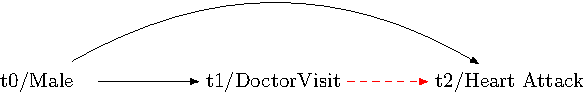
\includegraphics[width=0.8\textwidth,height=\textheight]{ow-methods_files/figure-pdf/fig-dag-1-1.pdf}

}

\caption{\label{fig-dag-1}Causal diagram adapted from Vanderweele et
al.'s three-wave panel design. The dotted line indicates a reduction in
bias arising from including baseline measures for the exposure and
outcome. For an unmeasured confounder U to bias the exposure-outcome
association, it would need to do so independently of these outcome and
exposure baseline measures. The graph clarifies that by measuring
confounders before the exposure and the exposure before the outcome, we
reduce the potential for reverse causation, collider stratification, and
mediator biases.}

\end{figure}

\hypertarget{step-3.-identify-observable-common-causes-of-the-exposure-and-the-outcome}{%
\subsubsection{Step 3. Identify observable common causes of the exposure
and the
outcome}\label{step-3.-identify-observable-common-causes-of-the-exposure-and-the-outcome}}

Next, we should identify all the potential confounders that, when
adjusted for, can eliminate any non-causal association between the
exposure and outcome. We should group these confounders under standard
labels wherever they share the same functional dependencies in the
graph. In a three-wave panel design, confounders are recorded during the
baseline wave. As illustrated in \textbf{?@fig-dag-mediator-solution},
recording confounders before the occurrence of the exposure minimises
the potential for mediation bias. For example in \textbf{?@fig-dag-6},
the variable \(L\) on the graph might denote rich set of indicators such
as Age, Gender, Education,Political Orientation, SES,\(\dots\) Again,
causal diagrams are meant to be human read. We should not include these
additional nodes when including a single node will suffice for clarity
and thoroughness.

\hypertarget{step-4.-gather-data-for-proxy-variables-of-unmeasured-common-causes-at-the-baseline-wave}{%
\subsubsection{Step 4. Gather data for proxy variables of unmeasured
common causes at the baseline
wave}\label{step-4.-gather-data-for-proxy-variables-of-unmeasured-common-causes-at-the-baseline-wave}}

Recall \textbf{?@fig-dag-descendent-solution-2}: if any unmeasured
confounders influence both the exposure and outcome, but we lack direct
measurements, we should make efforts to include proxies for them. Again,
even if this strategy cannot eliminate all bias from unmeasured
confounding, it will generally reduce bias.

\hypertarget{step-5.-state-the-target-population-for-whom-the-causal-question-applies}{%
\subsubsection{Step 5. State the target population for whom the causal
question
applies}\label{step-5.-state-the-target-population-for-whom-the-causal-question-applies}}

We need to define for whom our causal inference applies. For this
purpose, it is helpful to distinguish the concepts of source population
and target population and between the concepts of generalisability and
transportability.

\begin{enumerate}
\def\labelenumi{\arabic{enumi}.}
\item
  \textbf{The source population} is the population from whom our sample
  is drawn.
\item
  \textbf{The target population} is the larger population for whom we
  aim to apply our study's results. The closer the source population
  matches the target population in structural features relevant to our
  causal questions, the stronger our causal inferences about the target
  population will be.
\item
  \textbf{generalisability}: when the causal effect estimated from a
  sample applies to the target population beyond the sample population,
  we say the causal effect estimates are generalisable. This concept is
  also known as ``external validity.''
\end{enumerate}

Let \(PATE\) denote the population average treatment effect for the
target population. Let \(ATE_{\text{source}}\) denote the average
treatment effect in the source population. Let \(W\) denote a set of
variables upon which the source and target population structurally
differ. We say that results \emph{generalise} if there is a function
such that

\[PATE =  f(ATE_{\text{source}}, W)\]

\begin{enumerate}
\def\labelenumi{\arabic{enumi}.}
\setcounter{enumi}{3}
\tightlist
\item
  \textbf{Transportability}: when causal effects estimates may
  generalise to different settings and populations from which the source
  population was sampled, we say effects are transportable. Where \(T\)
  denotes a set of variables upon which the source and the target
  population structurally differ, we say that results are transportable
  if there is a function such that
\end{enumerate}

\[ATE_{\text{target}} \approx f(ATE_{\text{source}}, T)\]

This function similarly maps the average treatment effect from the
source population to a target population. The function over \(T\) might
be more complex, as it must handle potential heterogeneity of effects
and unobserved sources of bias. To assess transportability, we generally
require information about the source and target populations and a
specialist understanding. In Section 4, we will return to the concepts
of generalisability and transportability as they pertain to sample
selection.

\hypertarget{step-6.-retention-is-a-mission-critical-imperative}{%
\subsubsection{Step 6. Retention is a mission-critical
imperative}\label{step-6.-retention-is-a-mission-critical-imperative}}

for reasons we clarify in Part 4, sample retention is a mission-critical
imperative because panel attrition opens novel pathways for bias.
Researchers must develop protocols for tracking individuals as they
change addresses, emails, phone numbers, and names. Moreover, developing
and implementing strategies for motivating retention across the entire
population of interest (not merely those willing to volunteer for
science) is critical for causal human science. These strategies must be
developed with specialist knowledge of the population under study and
the participation and insights of the people being studied.

\hypertarget{part-2.-the-steps}{%
\subsection{Part 2. The Steps}\label{part-2.-the-steps}}

\hypertarget{step-1-formulate-the-research-question}{%
\subsubsection{STEP 1 Formulate the Research
Question}\label{step-1-formulate-the-research-question}}

\begin{itemize}
\tightlist
\item
  \textbf{Stating the Question:} Is my question clearly stated? If not,
  state it.
\item
  \textbf{Relevance of the Question:} Have I explained its importance?
  If not, explain.
\item
  \textbf{Ethical Considerations} How might this question affect people?
  How might not investigating this question affect people?
\item
  \textbf{Causality of the Question:} Is my question causal? If not,
  refine your question.
\item
  \textbf{Subgroup Analysis:} Does my question involve a subgroup (e.g.,
  cultural group)? If not, develop a subgroup analysis question.
\item
  \textbf{Understanding the Framework:} Can I explain the potential
  outcomes framework, individual causal effects, the experimental method
  to obtain average causal effects, the fundamental assumptions of
  causal inference, and the estimation of causal effects in
  observational data? If not, review course materials.
\end{itemize}

\hypertarget{data-requirements}{%
\subsubsection{Data Requirements}\label{data-requirements}}

\begin{itemize}
\tightlist
\item
  \textbf{Type of Data:} Are my data experimental? If yes, your project
  may not fit this course.
\item
  \textbf{Time-Series Data:} Are my data time-series? If not, reconsider
  your causal question.
\item
  \textbf{Data Waves:} Do I have at least three waves of data? If not,
  beware of confounding control issues.
\item
  \textbf{Data Source:} Are my data from the NZAVS simulated data set?
  If not, consult with me.
\end{itemize}

\hypertarget{defining-the-outcome}{%
\subsubsection{Defining the Outcome}\label{defining-the-outcome}}

\begin{itemize}
\tightlist
\item
  \textbf{Outcome Variable:} Is the outcome variable \emph{Y} defined?
  If not, define it.
\item
  \textbf{Multiple Outcomes:} Are there multiple outcomes? If yes, write
  them down.
\item
  \textbf{Outcome Relevance:} Can I explain how the outcome variable/s
  relate to my question? If not, clarify.
\item
  \textbf{Outcome Type:} Is my outcome binary and rare? If yes, consider
  logistic regression. If my outcome is continuous, consider
  z-transforming it or categorising it (consult an expert).
\item
  \textbf{Outcome Timing:} Does the outcome appear after the exposure?
  It should.
\end{itemize}

\hypertarget{determining-the-exposure}{%
\subsubsection{Determining the
Exposure}\label{determining-the-exposure}}

\begin{itemize}
\tightlist
\item
  \textbf{Exposure Variable:} Is the exposure variable \emph{A} defined?
  If not, define it.
\item
  \textbf{Multiple Exposures:} Are there multiple exposures? If yes,
  reassess; if only one exposure, proceed.
\item
  \textbf{Exposure Relevance:} Can I explain how the exposure variable
  relates to my question? If not, clarify.
\item
  \textbf{Positivity:} Can we intervene on the exposure at all levels of
  the covariates? We should be able to.
\item
  \textbf{Consistency:} Can I interpret what it means to intervene on
  the exposure? I should be able to.
\item
  \textbf{Exchangeability:} Are different versions of the exposure
  conditionally exchangeable given measured baseline confounders? They
  should be.
\item
  \textbf{Exposure Type:} Is the exposure binary or continuous? If
  continuous, z-transform it or consider categorising it (consult an
  expert).
\item
  \textbf{Exposure Timing:} Does the exposure appear before the outcome?
  It should.
\end{itemize}

\hypertarget{accounting-for-confounders}{%
\subsubsection{Accounting for
Confounders}\label{accounting-for-confounders}}

\begin{itemize}
\tightlist
\item
  \textbf{Baseline Confounders:} Have I defined my baseline confounders
  \emph{L}? I should have.
\item
  \textbf{Justification:} Can I explain how the baseline confounders
  could affect both \emph{A} and \emph{Y}? I should be able to.
\item
  \textbf{Timing:} Are the baseline confounders measured before the
  exposure? They should be.
\item
  \textbf{Inclusion:} Is the baseline measure of the exposure and the
  baseline outcome included in the set of baseline confounders? They
  should be.
\item
  \textbf{Sufficiency:} Are the baseline confounders sufficient to
  ensure balance on the exposure, such that \emph{A} is independent of
  \emph{Y} given \emph{L}? If not, plan a sensitivity analysis.
\item
  \textbf{Confounder Type:} Are the confounders continuous or binary? If
  so, consider converting them to z-scores. If they are categorical with
  three or more levels, do not convert them to z-scores.
\end{itemize}

\hypertarget{drawing-a-causal-diagram-with-unmeasured-confounders}{%
\subsubsection{Drawing a Causal Diagram with Unmeasured
Confounders}\label{drawing-a-causal-diagram-with-unmeasured-confounders}}

\begin{itemize}
\tightlist
\item
  \textbf{Unmeasured Confounders:} Does previous science suggest the
  presence of unmeasured confounders? If not, expand your understanding.
\item
  \textbf{Causal Diagram:} Have I drawn a causal diagram (DAG) to
  highlight both measured and unmeasured sources of confounding? I
  should have.
\item
  \textbf{M-Bias:} Have I considered the possibility of M-Bias? If not
  familiar, we'll discuss later.
\item
  \textbf{Measurement Error:} Have I described potential biases from
  measurement errors? If not, we'll discuss later.
\item
  \textbf{Temporal Order:} Does my DAG have time indicators to ensure
  correct temporal order? It should.
\item
  \textbf{Time Consistency:} Is my DAG organized so that time follows in
  a consistent direction? It should.
\end{itemize}

\hypertarget{identifying-the-estimand}{%
\subsubsection{Identifying the
Estimand}\label{identifying-the-estimand}}

\begin{itemize}
\tightlist
\item
  \textbf{Causal Estimand:} Is my causal estimand one of the following:
\end{itemize}

\[ATE_{G,(A,A')} = E[Y(1) - Y(0)|G, L]\]

\[ATE_{G,(A/A')} = \frac{E[Y(1)|G, L]}{E[Y(0)|G, L]}\]

If yes, you're on the right track.

\hypertarget{understanding-source-and-target-populations}{%
\subsubsection{Understanding Source and Target
Populations}\label{understanding-source-and-target-populations}}

\begin{itemize}
\tightlist
\item
  \textbf{Populations Identified:} Have I differentiated between my
  source and target populations? I should have.
\item
  \textbf{Generalisability and Transportability:} Have I considered
  whether my results generalise to the source population and transport
  to a different population? I should have.
\end{itemize}

\hypertarget{setting-eligibility-criteria}{%
\subsubsection{Setting Eligibility
Criteria}\label{setting-eligibility-criteria}}

\begin{itemize}
\tightlist
\item
  \textbf{Criteria Stated:} Have I stated the eligibility criteria for
  the study? I should have.
\end{itemize}

\hypertarget{describing-sample-characteristics}{%
\subsubsection{Describing Sample
Characteristics}\label{describing-sample-characteristics}}

\begin{itemize}
\tightlist
\item
  \textbf{Descriptive Statistics:} Have I provided descriptive
  statistics for demographic information taken at baseline? I should
  have.
\item
  \textbf{Exposure Change:} Have I demonstrated the magnitudes of change
  in the exposure from baseline to the exposure interval? I should have.
\item
  \textbf{References:} Have I included references for more information
  about the sample? I should have.
\end{itemize}

\hypertarget{addressing-missing-data}{%
\subsubsection{Addressing Missing Data}\label{addressing-missing-data}}

\begin{itemize}
\tightlist
\item
  \textbf{Missing Data Check:} Have I checked for missing data? I should
  have.
\item
  \textbf{Missing Data Plan:} If there is missing data, have I described
  how I will address it? I should have.
\end{itemize}

\hypertarget{selecting-the-model-approach}{%
\subsubsection{Selecting the Model
Approach}\label{selecting-the-model-approach}}

\begin{itemize}
\tightlist
\item
  \textbf{Approach Decision:} Have I decided on using G-computation,
  IPTW, or Doubly-Robust Estimation? I should have.
\item
  \textbf{Interaction Inclusion:} Have I included the interaction of the
  exposure and baseline covariates? I should have.
\item
  \textbf{Large Data Set:} If I have a large data set, should I include
  the interaction of the exposure, group, and baseline confounders? I
  should consider it.
\item
  \textbf{Model Specification:} Have I double-checked the model
  specification? I should.
\item
  \textbf{Outcome Specifics:} If the outcome is rare and binary, have I
  specified logistic regression? If it's continuous, have I considered
  converting it to z-scores?
\item
  \textbf{Sensitivity Analysis:} Am I planning a sensitivity analysis
  using simulation? If yes, describe it (e.g.~E-values.)
\end{itemize}

\hypertarget{d.-highlight-unmeasured-pre-treatment-covariates}{%
\subsubsection{d.~Highlight unmeasured pre-treatment
covariates}\label{d.-highlight-unmeasured-pre-treatment-covariates}}

Let \textbf{U} denoted unmeasured pre-treatment covariates that may
potentially bias the statistical association between \emph{A} and
\emph{Y} independently of the measured covariates.

\hypertarget{consider}{%
\subsubsection{Consider:}\label{consider}}

\begin{itemize}
\tightlist
\item
  To affect \emph{Y} and \emph{A}, \emph{U} must occur before \emph{A}.
\item
  It is useful to draw a causal diagramme to illustrate all potential
  sources of bias.
\item
  Causal diagrammes are qualitative tools that require specialist
  expertise. We cannot typically obtain a causal graph from the data.
\item
  A causal diagramme should include only as much information as is
  required to assess confounding. See Figure~\ref{fig-dag-outcomewide}
  for an example.
\item
  Because we cannot ensure the absence of unmeasured confounders in
  observational settings, it is vital to conduct sensitivity analyses
  for the results. For sensitivity analyeses, we use E-values, a topic
  for a latter seminar.
\end{itemize}

\begin{figure}

{\centering \includegraphics[width=1\textwidth,height=\textheight]{ow-methods_files/figure-pdf/fig-dag-outcomewide-1.pdf}

}

\caption{\label{fig-dag-outcomewide}Causal graph: three-wave panel
design.}

\end{figure}

\hypertarget{summary-step-1-consider-how-much-we-need-to-do-when-asking-a-causal-question}{%
\subsubsection{Summary Step 1: Consider how much we need to do when
asking a causal
question!}\label{summary-step-1-consider-how-much-we-need-to-do-when-asking-a-causal-question}}

We discover that asking a causal question is a multifaceted task. It
demands careful definition of the outcome, including its timing, the
exposure, and covariates. It also requires selecting the appropriate
scale for causal contrast, controlling for confounding, and potentially
adjusting for sample weights or stratification. Finally, when asking a
causal question, we must consider for whom the results apply. Only after
following these steps can we then ask: ``How may we answer this causal
question?''

\hypertarget{step-2-answer-a-causal-question}{%
\subsection{STEP 2: ANSWER A CAUSAL
QUESTION}\label{step-2-answer-a-causal-question}}

\hypertarget{obtain-longitudinal-data}{%
\paragraph{Obtain longitudinal data}\label{obtain-longitudinal-data}}

Note that causal inference from observational data turns on the
appropriate temporal ordering of the key variables involved in the
study.

Recall we have defined.

\begin{itemize}
\item
  \textbf{A}: Our exposure or treatment variable, denoted as \textbf{A}.
  Here we consider the example of `Church attendance'.
\item
  \textbf{Y}: The outcome variable we are interested in, represented by
  \textbf{Y}, is psychological distress. We operationalise this variable
  through the `Kessler-6' distress scale.
\item
  \textbf{L}: The confounding variables, collectively referred to as
  \textbf{L}, represent factors that can independently influence both
  \textbf{A} and \textbf{Y}. For example, socio-economic status could be
  a confounder that impacts both the likelihood of church attendance and
  the levels of psychological distress.
\end{itemize}

Given the importance of temporal ordering, we must now define time:

\begin{itemize}
\tightlist
\item
  \textbf{t} \(\in\) T: Let \(t\) denote within a multiwave panel study
  with \textbf{T} measurement intervals.
\end{itemize}

Where \(t/\text{{exposure}}\) denotes the measurement interval for the
exposure. Longitudinal data collection provides us the ability to
establish a causal model such that:

\[t_{confounders} < t_{exposure}< t_{outcome}\]

To minimise the posibility of time-varying confounding and obtain the
clearest effect estimates, we should acquire the most recent values of
\(\mathbf{L}\) preceding \(A\) and the latest values of \(A\) before
\(Y\).

Note in Figure~\ref{fig-dag-outcomewide}, We use the prefixes ``t0, t1,
and t2'' to denote temporal ordering. We include in the set of baseline
confounders the pre-exposure measurement of \emph{A} and \emph{Y}. This
allows for more substantial confounding control. For unmeasured
confounder to affect both the exposure and the outcome, it would need to
do so independently of the pre-exposure confounders. Additionally,
including the baseline exposure gives us an effect estimate for the
incidence exposure, rather than the prevelance of the exposure. This
helps us to assess the expected change in the outcome were we to initate
a change in the exposure.

\hypertarget{include-the-measured-exposure-with-baseline-covariates}{%
\subsubsection{Include the measured exposure with baseline
covariates}\label{include-the-measured-exposure-with-baseline-covariates}}

Controlling for prior exposure enables the interpretation of the effect
estimate as a change in the exposure in a manner akin to a randomised
trial. We propose that the effect estimate with prior control for the
exposure estimates the ``incidence exposure'' rather than the
``prevalence exposure'' (\protect\hyperlink{ref-danaei2012}{Danaei
\emph{et al.} 2012}). It is crucial to estimate the incidence exposure
because if the effects of an exposure are harmful in the short term such
that these effects are not subsequently measured, a failure to adjust
for prior exposure will yield the illusion that the exposure is
beneficial. Furthermore, this approach aids in controlling for
unmeasured confounding. For such a confounder to explain away the
observed exposure-outcome association, it would need to do so
independently of the prior level of the exposure and outcome.

\hypertarget{state-the-eligibility-criteria-for-participation}{%
\subsubsection{State the eligibility criteria for
participation}\label{state-the-eligibility-criteria-for-participation}}

This step is invaluable for assessing whether we are answering the
causal question that we have asked.

\hypertarget{consider-1}{%
\paragraph{Consider:}\label{consider-1}}

\begin{itemize}
\tightlist
\item
  Generalisability: we cannot evaluate inferences to a target group from
  the source population if we do not describe the source population
\item
  Eligibility criteria will help us to ensure whether we have correctly
  evaluated potential measurement bias/error in our instruments.
\end{itemize}

For example, the New Zealand Attitudes and Values Study is a National
Probability study of New Zealanders. The details provided in the
supplementary materials describe how individuals were randomly selected
from the country's electoral roll. From these invitations there was
typically less than 15\% response rate. How might this process of
recruitment affect generalisability and transportability of our results?

\begin{itemize}
\tightlist
\item
  Aside: discuss per protocol effects/ intention to treat effects
\end{itemize}

\hypertarget{determine-how-missing-data-will-be-handled}{%
\subsubsection{Determine how missing data will be
handled}\label{determine-how-missing-data-will-be-handled}}

\begin{itemize}
\tightlist
\item
  As we will consider in the upcoming weeks, loss to follow up and
  non-response opens sources for bias. We must develop a strategy for
  handling missing data.
\end{itemize}

\hypertarget{state-a-statistical-model}{%
\subsubsection{State a statistical
model}\label{state-a-statistical-model}}

The models we have considered in this course are G-computation, Inverse
Probability of Treatement Weighting, and Doubly-Robust estimation.

\hypertarget{reporting}{%
\subsubsection{Reporting}\label{reporting}}

Consider the following ideas about how to report one's model:

\begin{itemize}
\tightlist
\item
  \textbf{Estimator}: Doubly robust where possible.
\item
  \textbf{Propensity Score Reporting:} Detail the process of propensity
  score derivation, including the model used and any variable
  transformations.
\item
  \textbf{WeightIt Package Utilisation:} Explicitly mention the use of
  the `WeightIt' package in R, including any specific options or
  parameters used in the propensity score estimation process.
\item
  \textbf{Method Variations:} Report if different methods were used to
  obtain propensity scores, and the reasons behind the choice of methods
  such as `ebal', `energy', and `ps'.
\item
  \textbf{Continuous Exposures:} Highlight that for continuous
  exposures, only the `energy' option was used for propensity score
  estimation.
\item
  \textbf{Subgroup Estimation:} Confirm that the propensity scores for
  subgroups were estimated separately, and discuss how the weights were
  subsequently combined with the original data.
\item
  \textbf{Covariate Balance:} Include a Love plot to visually represent
  covariate balance on the exposure both before and after weighting.
\item
  \textbf{Weighting Algorithm Statistics:} Report the statistics for the
  weighting algorithms as provided by the WeightIt package, including
  any measures of balance or fit.
\item
  \textbf{Outcome Regression Model:} Clearly report the type of
  regression model used to estimate outcome model coefficients (e.g.,
  linear regression, Poisson, binomial), and mention if the exposure was
  interacted with the baseline covariates. Do not report model
  coefficients as these have no interpretation.
\item
  \textbf{Subgroup Interaction:} Address whether the subgroup was
  included separately as an interaction in the outcome model, and if the
  model successfully converged.
\item
  \textbf{Model Coefficients:} Note that the model coefficients should
  not be interpreted, as they are not meaningful in this context.
\item
  \textbf{Confidence Intervals and Standard Errors:} Describe the
  methods used to derive confidence intervals and standard errors,
  noting the use of the `clarify' package in R for simulation based
  inference.
\end{itemize}

\hypertarget{example-of-how-to-report-a-doubly-robust-method-in-your-report}{%
\subsubsection{Example of how to report a doubly robust method in your
report}\label{example-of-how-to-report-a-doubly-robust-method-in-your-report}}

The Doubly Robust Estimation method for Subgroup Analysis Estimator is a
sophisticated tool combining features of both IPTW and G-computation
methods, providing unbiased estimates if either the propensity score or
outcome model is correctly specified. The process involves five main
steps:

\textbf{Step 1} involves the estimation of the propensity score, a
measure of the conditional probability of exposure given the covariates
and the subgroup indicator. This score is calculated using statistical
models such as logistic regression, with the model choice depending on
the nature of the data and exposure. Weights for each individual are
then calculated using this propensity score. These weights depend on the
exposure status and are computed differently for exposed and unexposed
individuals. The estimation of propensity scores is performed separately
within each subgroup stratum.

\textbf{Step 2} focuses on fitting a weighted outcome model, making use
of the previously calculated weights from the propensity scores. This
model estimates the outcome conditional on exposure, covariates, and
subgroup, integrating the weights into the estimation process. Unlike in
propensity score model estimation, covariates are included as variables
in the outcome model. This inclusion makes the method doubly robust -
providing a consistent effect estimate if either the propensity score or
the outcome model is correctly specified, thereby reducing the
assumption of correct model specification.

\textbf{Step 3} entails the simulation of potential outcomes for each
individual in each subgroup. These hypothetical scenarios assume
universal exposure to the intervention within each subgroup, regardless
of actual exposure levels. The expectation of potential outcomes is
calculated for each individual in each subgroup, using
individual-specific weights. These scenarios are performed for both the
current and alternative interventions.

\textbf{Step 4} is the estimation of the average causal effect for each
subgroup, achieved by comparing the computed expected values of
potential outcomes under each intervention level. The difference
represents the average causal effect of changing the exposure within
each subgroup.

\textbf{Step 5} involves comparing differences in causal effects across
groups by calculating the differences in the estimated causal effects
between different subgroups. Confidence intervals and standard errors
for these calculations are determined using simulation-based inference
methods (\protect\hyperlink{ref-greifer2023}{Greifer \emph{et al.}
2023}). This step allows for a comprehensive comparison of the impact of
different interventions across various subgroups, while encorporating
uncertainty.

\hypertarget{inference}{%
\subsubsection{Inference}\label{inference}}

Consider the following ideas about what to discuss in one's findings.
The order of exposition might be different.

\begin{enumerate}
\def\labelenumi{\arabic{enumi}.}
\item
  \textbf{Summary of results}: What did you find?
\item
  \textbf{Interpretation of E-values:} Interpret the E-values used for
  sensitivity analysis. State what they represent in terms of the
  robustness of the findings to potential unmeasured confounding.
\item
  \textbf{Causal Effect Interpretation:} What is the interest of the
  effect, if any, if an effect was observed? Interpret the average
  causal effect of changing the exposure level within each subgroup, and
  discuss its relevance to the research question.
\item
  \textbf{Comparison of Subgroups:} Discuss how differences in causal
  effect estimates between different subgroups, if observed, or if not
  observed, contribute to the overall findings of the study.
\item
  \textbf{Uncertainty and Confidence Intervals:} Consider the
  uncertainty around the estimated causal effects, and interpret the
  confidence intervals to understand the precision of the estimates.
\item
  \textbf{Generalisability and Transportability:} Reflect on the
  generalizability of the study results to other contexts or
  populations. Discuss any factors that might influence the
  transportability of the causal effects found in the study. (Again see
  lecture 9.)
\item
  \textbf{Assumptions and Limitations:} Reflect on the assumptions made
  during the study and identify any limitations in the methodology that
  could affect the interpretation of results. State that the
  implications of different intervention levels on potential outcomes
  are not analysed.
\item
  \textbf{Theoretical Relevance}: How are these findings relevant to
  existing theories.
\item
  \textbf{Replication and Future Research:} Consider how the study could
  be replicated or expanded upon in future research, and how the
  findings contribute to the existing body of knowledge in the field.
\item
  \textbf{Real-world Implications:} Discuss the real-world implications
  of the findings, and how they could be applied in policy, practice, or
  further research.
\end{enumerate}

\hypertarget{part-x-estimators}{%
\subsection{Part X Estimators}\label{part-x-estimators}}

\hypertarget{average-treatment-effects-difference-scale}{%
\subsubsection{Average Treatment Effects (Difference
Scale)}\label{average-treatment-effects-difference-scale}}

\hypertarget{g-computation-estimator}{%
\subsubsection{\texorpdfstring{\textbf{G-computation
Estimator}}{G-computation Estimator}}\label{g-computation-estimator}}

\textbf{Step 1} Estimate the outcome model. Fit a model for the outcome
\(Y\), conditional on the exposure \(A\), and the covariates \(L\). This
model can be a linear regression, logistic regression, or another
statistical model. The goal is to capture the relationship between the
outcome, exposure, and confounders.

\[ \hat{E}(Y|A,L) = f_Y(A,L; \theta_Y) \]

This equation represents the expected value of the outcome \(Y\) given
the exposure \(A\), and covariates \(L\), as modeled by the function
\(f_Y\) with parameters \(\theta_Y\).

\textbf{Step 2} Simulate potential outcomes. For each individual,
predict their potential outcome under the intervention \(A=a\) using the
estimated outcome model:

\[\hat{E}(Y|A=a)  = \hat{E}[Y|A=a,L; \hat{\theta}_Y]\]

We also predict the potential outcome for everyone under the causal
contrast, setting the intervention to \(A=a'\):

\[  \hat{E}(Y|A=a')  = \hat{E}[Y|A=a',L; \hat{\theta}_Y]\]

In these equations, \(Y\) represents the potential outcome, \(A\) is the
intervention, and \(L\) are the covariates.

\textbf{Step 3} Calculate the estimated difference:

\[\hat{\delta} = \hat{E}[Y(a)] - \hat{E}[Y(a')]\]

This difference \(\hat{\delta}\) represents the average causal effect of
changing the exposure from level \(a'\) to level \(a\).

We use simulation-based inference methods to compute standard errors and
confidence intervals (\protect\hyperlink{ref-greifer2023}{Greifer
\emph{et al.} 2023}).

\hypertarget{inverse-probability-of-treatment-weighting-iptw-estimator}{%
\subsubsection{\texorpdfstring{\textbf{Inverse Probability of Treatment
Weighting (IPTW)
Estimator}}{Inverse Probability of Treatment Weighting (IPTW) Estimator}}\label{inverse-probability-of-treatment-weighting-iptw-estimator}}

\textbf{Step 1} Estimate the propensity score. The propensity score
\(e(L)\) is the conditional probability of the exposure \(A = 1\), given
the covariates \(L\). This can be modeled using logistic regression or
other suitable methods, depending on the nature of the data and the
exposure.

\[e = P(A = 1 | L) = f_A(L; \theta_A)\]

Here, \(f_A(L; \theta_A)\) is a function (statistical model) that
estimates the probability of the exposure \(A = 1\) given covariates
\(L\). Then, we calculate the weights for each individual, denoted as
\(v\):

\[
v = 
\begin{cases} 
\frac{1}{e} & \text{if } A = 1 \\
\frac{1}{1-e} & \text{if } A = 0 
\end{cases}
\]

\textbf{Step 2} Fit a weighted outcome model. Using the weights
calculated from the estimated propensity scores, fit a model for the
outcome \(Y\), conditional on the exposure \(A\):

\[ \hat{E}(Y|A; V) = f_Y(A; \theta_Y, V) \]

In this model, \(f_Y\) is a function (such as a weighted regression
model) with parameters \(\theta_Y\). The weights \(V\) are incorporated
into the estimation process, affecting how much each observation
contributes to the estimation.

\textbf{Step 3} Simulate potential outcomes. For each individual,
simulate their potential outcome under the hypothetical scenario where
everyone is exposed to the intervention \(A=a\):

\[\hat{E}(Y|A=a)  = \hat{E}[Y|A=a; \hat{\theta}_Y,  v_i]\]

and also under the hypothetical scenario where everyone is exposed to
intervention \(A=a'\):

\[\hat{E}(Y|A=a')  = \hat{E}[Y|A=a'; \hat{\theta}_Y,  v_i]\]

The expectation is calculated for each individual \(i\), with
individual-specific weights \(v_i\).

\textbf{Step 4} Estimate the average treatment effect as the difference
in the predicted outcomes:

\[\hat{\delta} = \hat{E}[Y(a)] - \hat{E}[Y(a')]\]

The estimated difference \(\hat{\delta}\) represents the ATE. We use
simulation-based inference methods to compute standard errors and
confidence intervals.

We again, use simulation-based inference methods to compute standard
errors and confidence intervals
(\protect\hyperlink{ref-greifer2023}{Greifer \emph{et al.} 2023}).

\hypertarget{doubly-robust-estimation}{%
\subsubsection{Doubly Robust
Estimation}\label{doubly-robust-estimation}}

\textbf{Step 1} Estimate the propensity score. The propensity score
\(e(L)\) is the conditional probability of the exposure \(A = 1\), given
the covariates \(L\).

\[e = P(A = 1 | L) = f_A(L; \theta_A)\]

Here, \(f_A(L; \theta_A)\) is a function (statistical model) estimating
the probability of exposure \(A = 1\) given covariates \(L\). We
calculate the weights for each individual, denoted as \(v\), using the
estimated propensity score:

\[
v = 
\begin{cases} 
\frac{1}{e} & \text{if } A = 1 \\
\frac{1}{1-e} & \text{if } A = 0 
\end{cases}
\]

\textbf{Step 2} Fit a weighted outcome model. Using the weights \(v\),
fit a model for the outcome \(Y\), conditional on the exposure \(A\).

\[ \hat{E}(Y|A, L; v) = f_Y(A, L ; \theta_Y, v) \]

Here, \(f_Y\) is a function (such as a weighted regression model) with
parameters \(\theta_Y\). The weights \(v\) are incorporated into the
estimation process.

\textbf{Step 3} Simulate potential outcomes under different scenarios
for each individual. For instance, simulate the outcome under the
hypothetical scenario where everyone is exposed to intervention \(A=a\):

\[\hat{E}(Y|A=a)  = \hat{E}[Y|A=a,L; \hat{\theta}_Y, v_i]\]

and also under the scenario where everyone is exposed to intervention
\(A=a'\):

\[\hat{E}(Y|A=a')  = \hat{E}[Y|A=a',L; \hat{\theta}_Y, v_i]\]

\textbf{Step 4} Estimate the average causal effect. Compute the
estimated expected value of the potential outcomes under each
intervention level:

\[\hat{\delta} = \hat{E}[Y(a)] - \hat{E}[Y(a')]\]

The difference \(\delta\) represents the average causal effect of
changing the exposure from level \(a^{\prime}\) to level \(a\).

We again use simulation-based inference methods to compute standard
errors and confidence intervals
(\protect\hyperlink{ref-greifer2023}{Greifer \emph{et al.} 2023}).

\hypertarget{subgroup-estimators}{%
\subsubsection{Subgroup estimators}\label{subgroup-estimators}}

\hypertarget{g-computation-for-subgroup-analysis-estimator}{%
\subsubsection{\texorpdfstring{\textbf{G-computation for Subgroup
Analysis
Estimator}}{G-computation for Subgroup Analysis Estimator}}\label{g-computation-for-subgroup-analysis-estimator}}

\textbf{Step 1} Estimate the outcome model. Fit a model for the outcome
\(Y\), conditional on the exposure \(A\), the covariates \(L\), and
subgroup indicator \(G\). This model can be a linear regression,
logistic regression, or another statistical model. The goal is to
capture the relationship between the outcome, exposure, confounders, and
subgroups.

\[ \hat{E}(Y|A,L,G) = f_Y(A,L,G; \theta_Y) \]

This equation represents the expected value of the outcome \(Y\) given
the exposure \(A\), covariates \(L\), and subgroup \(G\), as modeled by
the function \(f_Y\) with parameters \(\theta_Y\). This formulation
allows for the prediction of the average outcome \(Y\) given certain
values of \(A\), \(L\), and \(G\).

\textbf{Step 2} Simulate potential outcomes. For each individual in each
subgroup, predict their potential outcome under the intervention \(A=a\)
using the estimated outcome model:

\[\hat{E}(Y|A=a, G=g)  = \hat{E}[Y|A=a,L,G=g; \hat{\theta}_Y]\]

We also predict the potential outcome for everyone in each subgroup
under the causal contrast, setting the intervention for everyone in that
group to \(A=a'\):

\[\hat{E}(Y|A=a', G=g)  = \hat{E}[Y|A=a',L,G=g; \hat{\theta}_Y]\]

In these equations, \(Y\) represents the potential outcome, \(A\) is the
intervention, \(L\) are the covariates, \(G=g\) represents the subgroup,
and \(\theta_Y\) are the parameters of the outcome model.

\textbf{Step 3} Calculate the estimated difference for each subgroup
\(g\):

\[\hat{\delta}_g = \hat{E}[Y(a)|G=g] - \hat{E}[Y(a')|G=g]\]

This difference \(\hat{\delta}_g\) represents the average causal effect
of changing the exposure from level \(a'\) to level \(a\) within each
subgroup \(g\).

We use simulation-based inference methods to compute standard errors and
confidence intervals (\protect\hyperlink{ref-greifer2023}{Greifer
\emph{et al.} 2023}).

\textbf{Step 4} Compare differences in causal effects by subgroups:

\[\hat{\gamma} = \hat{\delta}_g - \hat{\delta}_{g'}\]

where,

\[\hat{\gamma} = \overbrace{\big( \hat{E}[Y(a)|G=g] - \hat{E}[Y(a^{\prime})|G=g] \big)}^{\hat{\delta_g}} - \overbrace{\big(\hat{E}[Y(a^{\prime})|G=g^{\prime}]- \hat{E}[Y(a)|G=g^{\prime}]\big)}^{\hat{\delta_{g^{\prime}}}}\]

This difference \(\hat{\gamma}\) represents the difference in the
average causal effects between the subgroups \(g\) and \(g'\). It
measures the interaction effect of the exposure \(A\) and the subgroup
\(G\) on the outcome \(Y\).

We again use simulation-based inference methods to compute standard
errors and confidence intervals
(\protect\hyperlink{ref-greifer2023}{Greifer \emph{et al.} 2023}).

\hypertarget{inverse-probability-of-treatment-weighting-iptw-for-subgroup-analysis-estimator}{%
\subsubsection{\texorpdfstring{\textbf{Inverse Probability of Treatment
Weighting (IPTW) for Subgroup Analysis
Estimator}}{Inverse Probability of Treatment Weighting (IPTW) for Subgroup Analysis Estimator}}\label{inverse-probability-of-treatment-weighting-iptw-for-subgroup-analysis-estimator}}

\textbf{Step 1} Estimate the propensity score. The propensity score
\(e(L, G)\) is the conditional probability of the exposure \(A = 1\),
given the covariates \(L\) and subgroup indicator \(G\). This can be
modeled using logistic regression or other suitable methods, depending
on the nature of the data and the exposure.

\[e = P(A = 1 | L, G) = f_A(L, G; \theta_A)\]

Here, \(f_A(L, G; \theta_A)\) is a function (statistical model) that
estimates the probability of the exposure \(A = 1\) given covariates
\(L\) and subgroup \(G\). Then, we calculate the weights for each
individual, denoted as \(v\), using the estimated propensity score:

\[
v = 
\begin{cases} 
\frac{1}{e} & \text{if } A = 1 \\
\frac{1}{1-e} & \text{if } A = 0 
\end{cases}
\]

Thus, \(v\) depends on \(A\), and is calculated as the inverse of the
propensity score for exposed individuals and as the inverse of \(1-e\)
for unexposed individuals.

Note that we estimate propensity scores \emph{separately} within strata
of the subgroup for whom we are interested in effect modification. \(v\)
is the weight for each individual in a given subgroup \(G\).

\textbf{Step 2} Fit a weighted outcome model. Using the weights
calculated from the estimated propensity scores, fit a model for the
outcome \(Y\), conditional on the exposure \(A\) and subgroup \(G\).
This can be represented as:

\[ \hat{E}(Y|A, G; V) = f_Y(A, G ; \theta_Y, V) \]

In this model, \(f_Y\) is a function (such as a weighted regression
model) with parameters \(θ_Y\). The weights \(V\) are incorporated into
the estimation process, affecting how much each observation contributes
to the estimation of \(θ_Y\), but they are not themselves an additional
variable within the model.

Note that in this formulation, unlike doubly-robust estimation, \(L\) is
not included as a variable in the outcome model, but its effect is
accounted for through the weights \(V\), which are calculated based on
the estimated propensity scores that do include \(L\).

\textbf{Step 3} Simulate potential outcomes. For each individual in each
subgroup, simulate their potential outcome under the hypothetical
scenario where everyone in the subgroup is exposed to the intervention
\(A=a\) regardless of their actual exposure level:

\[\hat{E}(Y|A=a, G=g)  = \hat{E}[Y|A=a,G=g; \hat{\theta}_Y,  v_i]\]

and also under the hypothetical scenario where everyone is exposed to
intervention \(A=a'\):

\[\hat{E}(Y|A=a', G=g)  = \hat{E}[Y|A=a',G=g; \hat{\theta}_Y,  v_i]\]

Thus the expectation is calculated for each individual \(i\) in each
subgroup \(g\), with individual-specific weights \(v_i\).

\textbf{Step 4} Estimate the average causal effect for each subgroup as
the difference in the predicted outcomes:

\[\hat{\delta}_g = \hat{E}[Y(a)|G=g] - \hat{E}[Y(a')|G=g]\]

The estimated difference \(\hat{\delta}_g\) represents the average
causal effect withing group \(g\). We use simulation-based inference
methods to compute standard errors and confidence intervals
(\protect\hyperlink{ref-greifer2023}{Greifer \emph{et al.} 2023}).

\textbf{Step 5} Compare differences in causal effects by groups. Compute
the differences in the estimated causal effects between different
subgroups:

\[\hat{\gamma} = \hat{\delta}_g - \hat{\delta}_{g'}\]

where,

\[\hat{\gamma} = \overbrace{\big( \hat{E}[Y(a)|G=g] - \hat{E}[Y(a^{\prime})|G=g] \big)}^{\hat{\delta_g}} - \overbrace{\big(\hat{E}[Y(a^{\prime})|G=g^{\prime}]- \hat{E}[Y(a)|G=g^{\prime}]\big)}^{\hat{\delta_{g^{\prime}}}}\]

We again use simulation-based inference methods to compute standard
errors and confidence intervals
(\protect\hyperlink{ref-greifer2023}{Greifer \emph{et al.} 2023}).

\hypertarget{doubly-robust-estimation-for-subgroup-analysis-estimator}{%
\subsubsection{Doubly Robust Estimation for Subgroup Analysis
Estimator}\label{doubly-robust-estimation-for-subgroup-analysis-estimator}}

Doubly Robust Estimation is a powerful technique that combines the
strengths of both the IPTW and G-computation methods. It uses both the
propensity score model and the outcome model, which makes it doubly
robust: it produces unbiased estimates if either one of the models is
correctly specified.

\textbf{Step 1} Estimate the propensity score. The propensity score
\(e(L, G)\) is the conditional probability of the exposure \(A = 1\),
given the covariates \(L\) and subgroup indicator \(G\). This can be
modeled using logistic regression or other suitable methods, depending
on the nature of the data and the exposure.

\[e = P(A = 1 | L, G) = f_A(L, G; \theta_A)\]

Here, \(f_A(L, G; \theta_A)\) is a function (statistical model) that
estimates the probability of the exposure \(A = 1\) given covariates
\(L\) and subgroup \(G\). Then, we calculate the weights for each
individual, denoted as \(v\), using the estimated propensity score:

\[
v = 
\begin{cases} 
\frac{1}{e} & \text{if } A = 1 \\
\frac{1}{1-e} & \text{if } A = 0 
\end{cases}
\]

Thus, \(v\) depends on \(A\), and is calculated as the inverse of the
propensity score for exposed individuals and as the inverse of \(1-e\)
for unexposed individuals.

Note that we estimate propensity scores \emph{separately} within strata
of the subgroup for whom we are interested in effect modification. \(v\)
is the weight for each individual in a given subgroup \(G\).

\textbf{Step 2} Fit a weighted outcome model. Using the weights
calculated from the estimated propensity scores, fit a model for the
outcome \(Y\), conditional on the exposure \(A\) and subgroup \(G\).
This can be represented as:

\[ \hat{E}(Y|A, L, G; V) = f_Y(A, L, G ; \theta_Y, V) \]

In this model, \(f_Y\) is a function (such as a weighted regression
model) with parameters \(θ_Y\). The weights \(V\) are incorporated into
the estimation process, affecting how much each observation contributes
to the estimation of \(θ_Y\), but they are not themselves an additional
variable within the model.

Note that in this formulation, unlike propensity score model,
estimation, \(L\) is included as a variable in the outcome model,
Although imbalance in \(L\) on \(A\) is accounted for by the weights
\(V\), by including \(L\) in the outcome model this method is doubly
robust insofar as we will obtain a consistent effect estimate if either
the propensity score or the outcome model is correctly specified. This
property reduces the strength of the assumption of correct model
specification.

\textbf{Step 3} For each individual in each subgroup, simulate their
potential outcome under the hypothetical scenario where everyone in the
subgroup is exposed to the intervention \(A=a\) regardless of their
actual exposure level:

\[\hat{E}(Y|A=a, G=g)  = \hat{E}[Y|A=a,L,G=g; \hat{\theta}_Y,  v_i]\]

and also under the hypothetical scenario where everyone in each subgroup
is exposed to intervention \(A=a'\):

\[\hat{E}(Y|A=a', G=g)  = \hat{E}[Y|A=a',L,G=g; \hat{\theta}_Y,  v_i]\]

Thus the expectation is calculated for each individual \(i\) in each
subgroup \(g\), with individual-specific weights \(v_i\).

\textbf{Step 4} Estimate the average causal effect for each subgroup.
Compute the estimated expected value of the potential outcomes under
each intervention level for each subgroup:

\[\hat{\delta}_g = \hat{E}[Y(a)|G=g] - \hat{E}[Y(a')|G=g]\]

The difference \(\delta_g\) represents the average causal effect of
changing the exposure from level \(a^{\prime}\) to level \(a\) within
each subgroup.

We use simulation-based inference methods to compute standard errors and
confidence intervals (\protect\hyperlink{ref-greifer2023}{Greifer
\emph{et al.} 2023}).

\textbf{Step 5} Compare differences in causal effects by groups. Compute
the differences in the estimated causal effects between different
subgroups:

\[\hat{\gamma} = \hat{\delta}_g - \hat{\delta}_{g'}\]

where,

\[\hat{\gamma} = \overbrace{\big( \hat{E}[Y(a)|G=g] - \hat{E}[Y(a^{\prime})|G=g] \big)}^{\hat{\delta_g}} - \overbrace{\big(\hat{E}[Y(a^{\prime})|G=g^{\prime}]- \hat{E}[Y(a)|G=g^{\prime}]\big)}^{\hat{\delta_{g^{\prime}}}}\]

We again use simulation-based inference methods to compute standard
errors and confidence intervals
(\protect\hyperlink{ref-greifer2023}{Greifer \emph{et al.} 2023}).

\hypertarget{refs}{}
\begin{CSLReferences}{1}{0}
\leavevmode\vadjust pre{\hypertarget{ref-bulbulia2022}{}}%
Bulbulia, JA (2022) A workflow for causal inference in cross-cultural
psychology. \emph{Religion, Brain \& Behavior}, \textbf{0}(0), 1--16.
doi:\href{https://doi.org/10.1080/2153599X.2022.2070245}{10.1080/2153599X.2022.2070245}.

\leavevmode\vadjust pre{\hypertarget{ref-chatton2020}{}}%
Chatton, A, Le Borgne, F, Leyrat, C, \ldots{} Foucher, Y (2020)
G-computation, propensity score-based methods, and targeted maximum
likelihood estimator for causal inference with different covariates
sets: a comparative simulation study. \emph{Scientific Reports},
\textbf{10}(1), 9219.
doi:\href{https://doi.org/10.1038/s41598-020-65917-x}{10.1038/s41598-020-65917-x}.

\leavevmode\vadjust pre{\hypertarget{ref-danaei2012}{}}%
Danaei, G, Tavakkoli, M, and Hernán, MA (2012) Bias in observational
studies of prevalent users: lessons for comparative effectiveness
research from a meta-analysis of statins. \emph{American Journal of
Epidemiology}, \textbf{175}(4), 250--262.
doi:\href{https://doi.org/10.1093/aje/kwr301}{10.1093/aje/kwr301}.

\leavevmode\vadjust pre{\hypertarget{ref-greifer2023}{}}%
Greifer, N, Worthington, S, Iacus, S, and King, G (2023) \emph{Clarify:
Simulation-based inference for regression models}. Retrieved from
\url{https://iqss.github.io/clarify/}

\leavevmode\vadjust pre{\hypertarget{ref-hernuxe1n2023}{}}%
Hernán, MA, and Monge, S (2023) Selection bias due to conditioning on a
collider. \emph{BMJ}, \textbf{381}, p1135.
doi:\href{https://doi.org/10.1136/bmj.p1135}{10.1136/bmj.p1135}.

\leavevmode\vadjust pre{\hypertarget{ref-hernuxe1n2016a}{}}%
Hernán, MA, Sauer, BC, Hernández-Díaz, S, Platt, R, and Shrier, I (2016)
Specifying a target trial prevents immortal time bias and other
self-inflicted injuries in observational analyses. \emph{Journal of
Clinical Epidemiology}, \textbf{79}, 7075.

\leavevmode\vadjust pre{\hypertarget{ref-hernuxe1n2022}{}}%
Hernán, MA, Wang, W, and Leaf, DE (2022) Target trial emulation: A
framework for causal inference from observational data. \emph{JAMA},
\textbf{328}(24), 2446--2447.
doi:\href{https://doi.org/10.1001/jama.2022.21383}{10.1001/jama.2022.21383}.

\leavevmode\vadjust pre{\hypertarget{ref-ogburn2021}{}}%
Ogburn, EL, and Shpitser, I (2021) Causal modelling: The two cultures.
\emph{Observational Studies}, \textbf{7}(1), 179--183.
doi:\href{https://doi.org/10.1353/obs.2021.0006}{10.1353/obs.2021.0006}.

\leavevmode\vadjust pre{\hypertarget{ref-shi2021}{}}%
Shi, B, Choirat, C, Coull, BA, VanderWeele, TJ, and Valeri, L (2021)
CMAverse: A suite of functions for reproducible causal mediation
analyses. \emph{Epidemiology}, \textbf{32}(5), e20e22.

\leavevmode\vadjust pre{\hypertarget{ref-vantongeren2020}{}}%
Van Tongeren, DR, DeWall, CN, Chen, Z, Sibley, CG, and Bulbulia, J
(2020) Religious residue: Cross-cultural evidence that religious
psychology and behavior persist following deidentification.
\emph{Journal of Personality and Social Psychology}.

\leavevmode\vadjust pre{\hypertarget{ref-vanderweele2020}{}}%
VanderWeele, TJ, Mathur, MB, and Chen, Y (2020) Outcome-wide
longitudinal designs for causal inference: A new template for empirical
studies. \emph{Statistical Science}, \textbf{35}(3), 437466.

\end{CSLReferences}



\end{document}
